\section{General overview}
The design of the User Interface for the BBP app has a vital role in ensuring a clear and friendly user experience. The following section contains a comprehensive look at the app and its core functionalities  through the use of a mock-up UI highlighting the features that make the app as intuitive and easy to use.

The UI features a clean and consistent layout, allowing users to quickly access core features easily and understand how to navigate each section without difficulty.

UI mock-ups are not provided for every page described in the DD document; only the most relevant sections and their functionalities are showcased. For simplicity, this document does not include pop ups, although some may be used in the app itself. 

Design choices, fonts and colors may be modified to follow business decisions to improve user engagement.

Each app screen is responsive and adapts to all user devices












\newpage
\section{User Interface Layouts}
\subsection{User Authentication}

\begin{figure}[ht]
    \centering
    \begin{minipage}{0.30\textwidth}
        \centering
        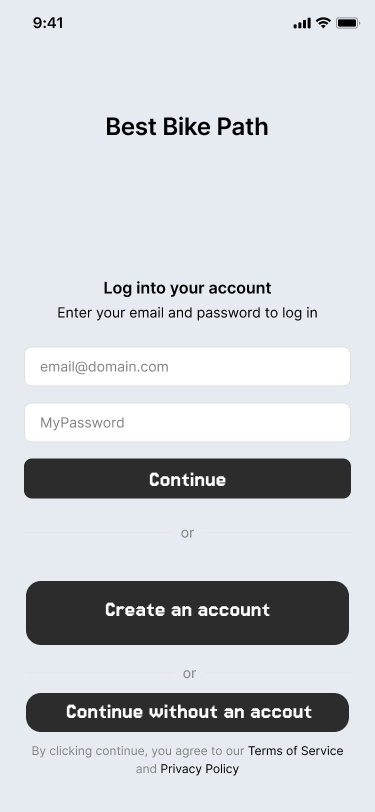
\includegraphics[width=\linewidth]{DD/Images/UI/Sign_In.png}
        \caption{Sign in}
    \end{minipage}
    \hspace{3cm}
    \begin{minipage}{0.30\textwidth}
        \centering
        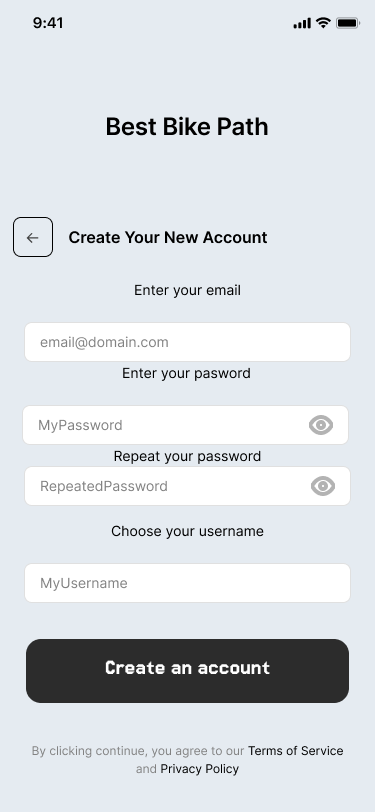
\includegraphics[width=\linewidth]{DD/Images/UI/Sign_Up.png}
        \caption{Sign up}
    \end{minipage}
\end{figure}


Figure 3.1 shows the screen displayed when a user opens the BBP app for the first time. From this screen, users can either log into an existing account by entering their credentials and pressing \textit{Continue}, or create a new account by selecting the \textit{Create an account} button. Alternatively, users may choose to access the application with limited functionalities by pressing \textit{Continue without an account}.

Figure 3.2 illustrates the account creation screen, where a user can create a new BBP account by providing all the required information and pressing \textit{Create an account}. If the user wishes to return to the sign-in screen, they can do so by pressing the arrow located in the top-left corner of the screen.


\newpage
\subsection{Map and navigation}
\begin{figure}[ht]
    \centering
    \begin{minipage}{0.30\textwidth}
        \centering
        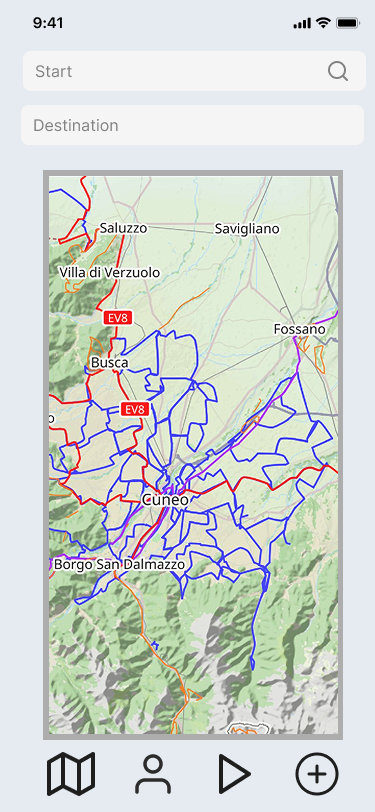
\includegraphics[width=\linewidth]{DD/Images/UI/Map 2.png}
        \caption{Map}
    \end{minipage}
    \hspace{3cm}
    \begin{minipage}{0.30\textwidth}
        \centering
        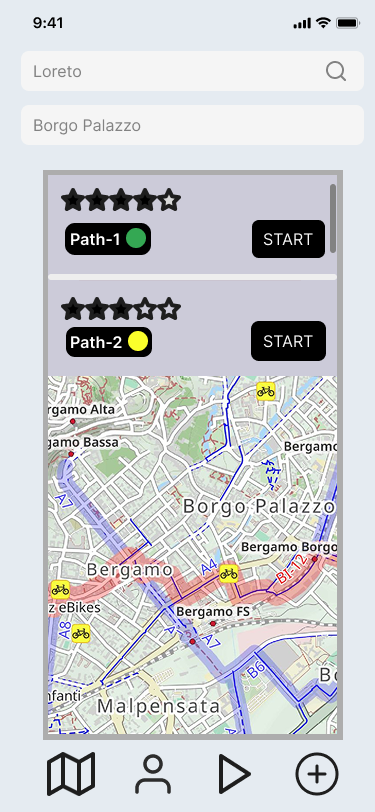
\includegraphics[width=\linewidth]{DD/Images/UI/Map 1.png}
        \caption{Navigation}
    \end{minipage}
\end{figure}

This section describes what a user sees after authentication, either when opening the app from the second time onward or by selecting the map icon in the bottom navigation bar. Figure 3.3 represents the standard map view, showing all the available bike paths in the selected area. The user can zoom in and out and move the map using touch gestures.

Figure 3.4 illustrates the navigation view displayed after the user specifies an origin and a destination using the search bar at the top of the screen. Below the map, the system presents the best available paths ranked according to their score, together with the corresponding score and average road quality. The top-ranked path is highlighted in red on the map. The user can start following a selected path by pressing \textit{Start} on the right side of the corresponding path entry.



\newpage
\subsection{Profile}
\begin{figure}[ht]
    \centering
    \begin{minipage}{0.30\textwidth}
        \centering
        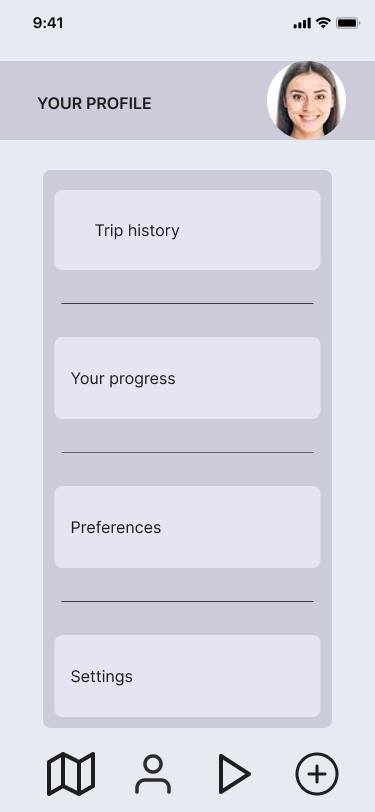
\includegraphics[width=\linewidth]{DD/Images/UI/Profile.png}
        \caption{Profile}
    \end{minipage}
    \hspace{0.5cm}
    \begin{minipage}{0.30\textwidth}
        \centering
        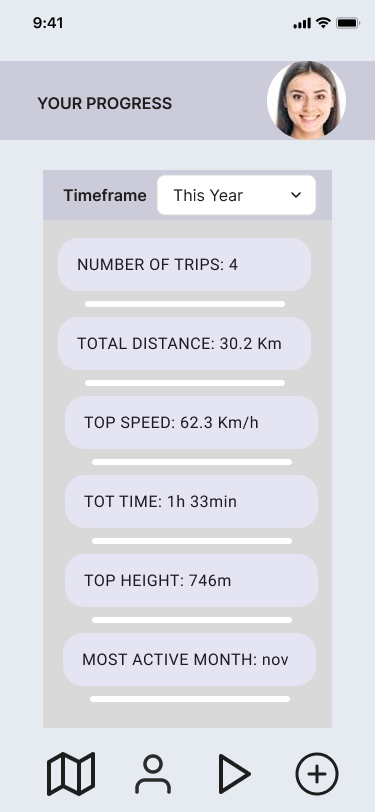
\includegraphics[width=\linewidth]{DD/Images/UI/Your Progress.png}
        \caption{Activity}
    \end{minipage}    
    \hspace{0.5cm}
    \begin{minipage}{0.30\textwidth}
        \centering
        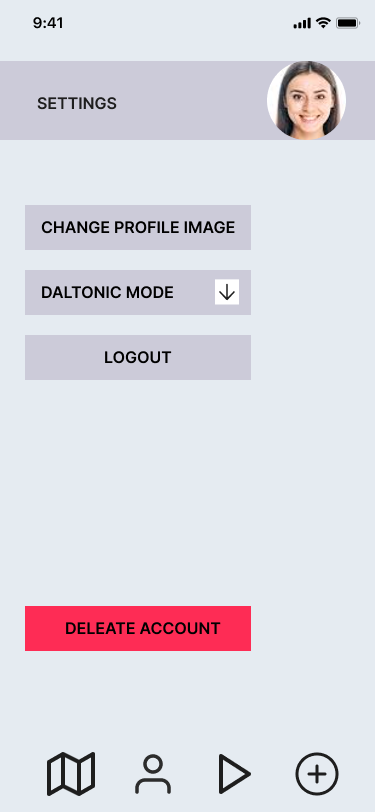
\includegraphics[width=\linewidth]{DD/Images/UI/Settings.png}
        \caption{Settings}
    \end{minipage}
\end{figure}

The profile interface can be accessed by selecting the human-shaped icon in the bottom navigation bar. From this screen, pressing the \textit{Trip history} button allows the user to access all information related to their recorded trips, including detailed statistics and the option to publish them.

As shown in Figure 3.6, by selecting \textit{Your progress} the user can view an overview of their activity, including metrics such as the total number of completed trips and the cumulative distance traveled. These statistics can be further filtered by a selected time frame, such as \textit{This year}.

The \textit{Preferences} section allows the user to specify preferred road types and disliked obstacles, enabling BBP to personalize the path scoring system and provide a more tailored user experience for registered users. As illustrated in Figure 3.7, by selecting \textit{Settings} the user can modify basic account settings, such as the profile image, or perform actions including logging out or deleting the account.


\newpage
\subsection{Trip history}
\begin{figure}[ht]
    \centering
    \begin{minipage}{0.30\textwidth}
        \centering
        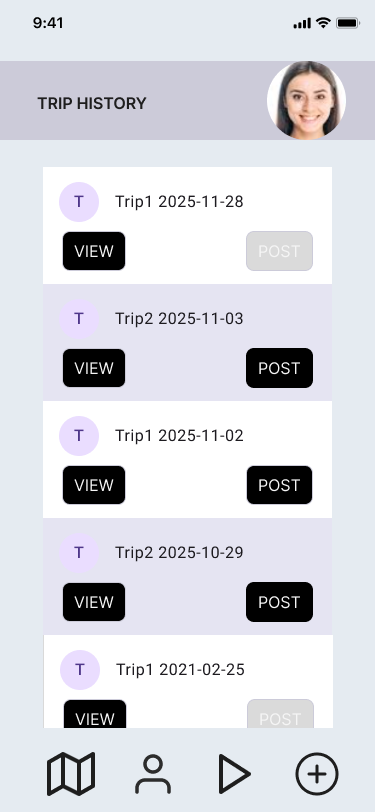
\includegraphics[width=\linewidth]{DD/Images/UI/Trip History.png}
        \caption{History}
    \end{minipage}
    \hspace{3cm}
    \begin{minipage}{0.30\textwidth}
        \centering
        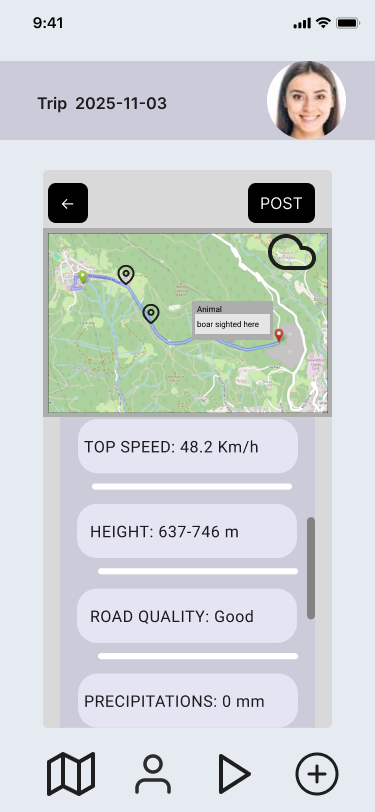
\includegraphics[width=\linewidth]{DD/Images/UI/Trip Visual2.png}
        \caption{Trip data}
    \end{minipage}
\end{figure}
Figure 3.8 shows the interface displayed when a user selects \textit{Trip history} from the profile section. From this screen, the user can view the list of all completed trips in chronological order. By pressing \textit{Post}, the user can publish the contributions associated with a trip; this button is disabled if the trip has already been published.

Figure 3.9 can be accessed by pressing \textit{View} on any trip in the history list. This screen displays detailed trip statistics together with a map representation of the recorded path. The pins shown on the map represent detected events, and the user can view their details by selecting the corresponding pin.


\newpage
\subsection{Automated trips}
\begin{figure}[ht]
    \centering
    \begin{minipage}{0.30\textwidth}
        \centering
        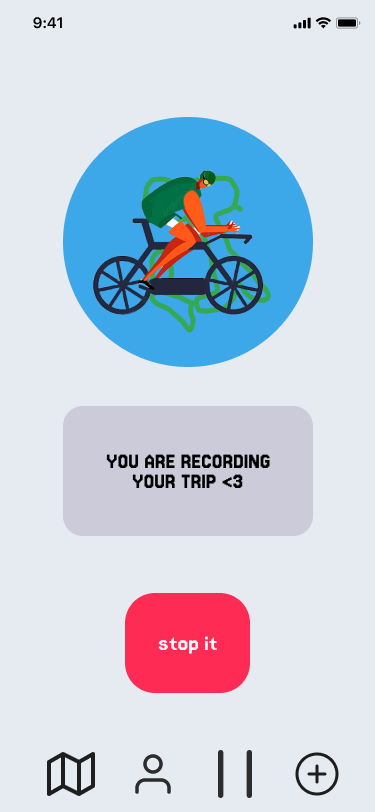
\includegraphics[width=\linewidth]{DD/Images/UI/Automatic 1.png}
        \caption{Trip recording}
    \end{minipage}
    \hspace{3cm}
    \begin{minipage}{0.30\textwidth}
        \centering
        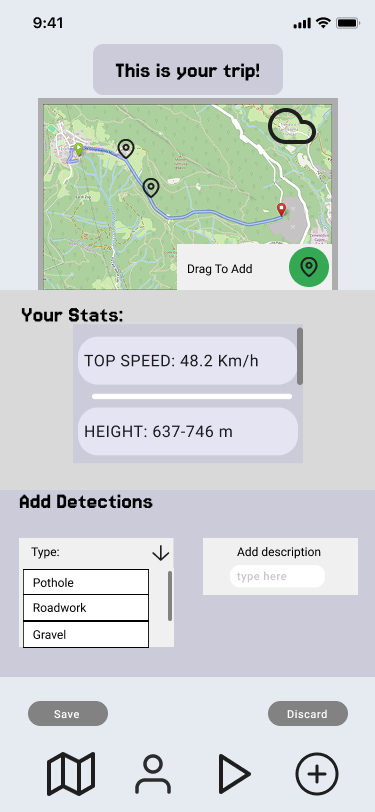
\includegraphics[width=\linewidth]{DD/Images/UI/Automatic 2.png}
        \caption{modify trip}
    \end{minipage}
\end{figure}
Figure~3.10 is displayed when a user selects the \textit{Play} icon in the bottom navigation bar, starting the automatic trip recording process, during which sensor data and trip statistics are collected. While the recording is active, the user can continue to use the other functionalities of the application. To stop the recording, the user can press the red \textit{Stop} button shown in Figure~3.10 or the same button used to start the recording from any screen.

After the trip is stopped, the user is presented with the interface shown in Figure~3.11, where all recorded statistics can be visualized and additional detections can be added by selecting a category and dragging a green pin to the desired location. Detections can also be removed by selecting them and pressing the \textit{X} button that appears. The user may then save the trip to their history, with the option to publish it immediately or at a later time, or discard the trip entirely by selecting the corresponding action.


\newpage
\subsection{Manual trip Insertion}
\begin{figure}[ht]
    \centering
    \begin{minipage}{0.30\textwidth}
        \centering
        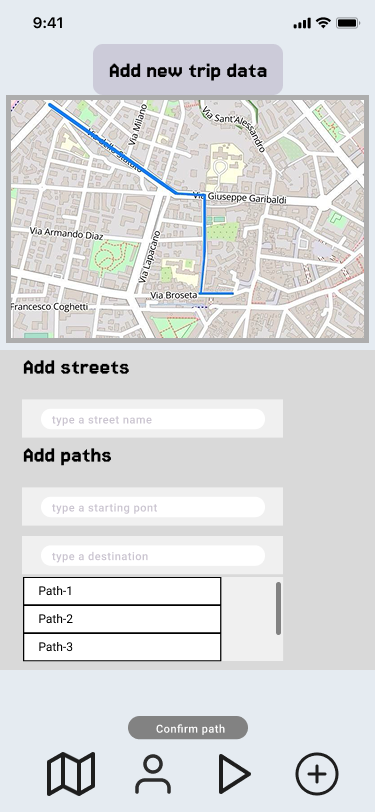
\includegraphics[width=\linewidth]{DD/Images/UI/Manual 1.png}
        \caption\protect\mbox{Path generation}
    \end{minipage}
    \hspace{3cm}
    \begin{minipage}{0.30\textwidth}
        \centering
        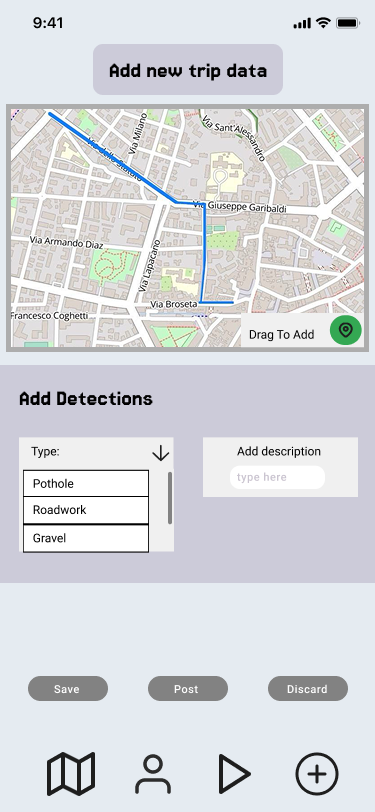
\includegraphics[width=\linewidth]{DD/Images/UI/Manual 2.png}
        \caption\protect\mbox{Detection generation}
    \end{minipage}
\end{figure}

Figure~3.12 is displayed when a user selects the \textit{+} button in the bottom navigation bar, initiating the manual trip creation process. From this screen, the user can add street segments by selecting them directly on the map, entering the name of a street, or searching for an entire path by specifying a starting point and a destination. Once the desired path is defined, it is displayed in blue, and the user can proceed by pressing the \textit{Confirm path} button.

After confirming the path, the interface shown in Figure~3.13 is displayed, allowing the user to add detections using the same interaction methods described in the previous section. Once all desired detections have been added, the user may save the trip to their history, publish it solely as a contribution without storing the trip in the history, or discard the trip entirely by selecting the corresponding option.
